\documentclass[12pt]{article}
\usepackage{fontspec}   %加這個就可以設定字體
\usepackage{xeCJK}       %讓中英文字體分開設置
\setmainfont{Times New Roman}
\setCJKmainfont{標楷體} %設定中文為系統上的字型,而英文不去更動,使用原TeX字型
\XeTeXlinebreaklocale "zh"             %這兩行一定要加,中文才能自動換行
\XeTeXlinebreakskip = 0pt plus 1pt     %這兩行一定要加,中文才能自動換行
\usepackage{amsmath, amsthm, amssymb} %引入數學符號的套件,例如實數R、定理Thm...
\usepackage{graphicx}                 %現在, 假設我們要插入 pic.png 這個圖檔, 使用
%\title{我是標題}
%\author{我是作者}
%\date{} %不要日期

\newcommand{\uA}       {\mbox{\boldmath$A$}}
\usepackage{textcomp}
\usepackage{array}
\usepackage{graphicx}
\usepackage{colortbl}
\usepackage{color,xcolor}
\usepackage{listings}
\usepackage{array,booktabs}   %這三個為表格使用的套件
\usepackage{textpos}
\usepackage{float}
\usepackage{listings}

\title{Statistical learning assignment 3 - ch 2$\thicksim$3}
\author{孫浩哲 \hspace{0.7cm} M072040002}
\date{October 4, 2018}
\begin{document}
\maketitle
%%%%%%%%%%%%%%%%%%%%%%%%%%%%%
\begin{itemize}
\item[\Large2-6.]
\ \\
\normalsize
Parametric approach:Assume a form for f by estimating a set of parameters.\\[3ex]
Non-parametric approach:Requires a very large number of observations to accurately estimate f.\\[3ex]
Advantages:simplifying of modeling f to a few parameters and it doesn't need large number of observations.\\[3ex]
Disadvantages:The assumption may be incorrect, overfitting if we use more flexible models.
%%%%%%%%%%%%%%%%%%%%%%%%%%%%%
\item[\Large2-7.]
\ \\
\normalsize
(a)\\[2ex]
\ obs.\ $1$:$\sqrt{0^2+3^2+0^2}=3$\\[2ex]
\ obs.\ $2$:$\sqrt{2^2+0^2+0^2}=2$\\[2ex]
\ obs.\ $3$:$\sqrt{0^2+1^2+3^2}=\sqrt{10}$\\[2ex]
\ obs.\ $4$:$\sqrt{0^+1^2+2^2}=\sqrt{5}$\\[2ex]
\ obs.\ $5$:$\sqrt{(-1)^2+0^2+1^2}=\sqrt{2}$\\[2ex]
\ obs.\ $6$:$\sqrt{1^2+1^2+1^2}=\sqrt{3}$\\[5ex]
(b)\\[2ex]
\ Green, because the obs.\ $5$ is the closest neighbor when $K=1$.\\[5ex]
(c)\\[2ex]
\ Red, because the most closest neighbors when\ $K=3$ are obs.\ $5$, obs.\ $6$ and obs.\ $2$, and they are Green, Red and Red.\\[5ex]
(d)\\[2ex]
\ Small, A small\ $K$ would be flexible for a non-linear decision boundary.\\
Large\ $K$ would try to fit a more linear boundary.
\item[\Large3-1.]
\ \\
\normalsize
\begin{table}[h]
  \raggedright
  \begin{tabular}{|c|c|c|}
  \hline
   predictors & null hypothesis &\ T/F \\
   \hline
   TV & TV ads have no effect on sales in the presence of radio and newspaper.& False \\
   \hline
   radio & radio ads have no effect on sales in the presence of TV and newspaper.& False\\
   \hline
   newspaper & newspaper ads have no effect on sales in the presence of TV and radio.&True\\
   \hline
  \end{tabular}
  \caption{null hypothesis for each predictor and True or False}
  \label{Table.1}
\end{table}
%%%%%%%%%%%%%%%%%%%%%%%%%%%%%
\item[\Large3-3.]
\ \\
Model that predict the starting salary:\\
$$ salary = 50 + 20(GPA) + 0.07(IQ) + 35(gender) + 0.01(GPA \times IQ) - 10 (GPA \times gender)$$\raggedright\\[3ex]
(a.)\\ Assume that GPA\ $=x_{0}$, IQ\ $=x_{1}$\\[2ex]
male(gender\ $=0$):
$$salary=50+20x_{0}+0.07x_{1}+0.01(x_{0}\times x_{1})$$\\
female(gender\ $=1$):
$$salary=85+20x_{0}+0.07x_{1}+0.01(x_{0} \times x_{1})-10x_{0}$$
It can't conclude which gender's salary is higher than another one unless the GPA\ $>3.5$.So we choose(iii.)\\[2ex]
(b.)
$$50+20 \times 4.0+0.07 \times 110 + 0.01 \times (4.0 \times 110)-10 \times 4.0 = 137.1$$
(c.)\\[3ex]
\ False, because we haven't examined the\ $p$-value of the null hypothesis correspond to the coefficient.
%%%%%%%%%%%%%%%%%%%%%%%%%%%%%
\item[\Large3-8.]
\ \\
\normalsize
\begin{verbatim}
library(ISLR)
auto=Auto
auto=na.omit(Auto)
summary(auto)
attach(auto)
model=lm(mpg~horsepower)
summary(model)

> summary(model)

Call:
lm(formula = mpg ~ horsepower)

Residuals:
     Min       1Q   Median       3Q      Max
-13.5710  -3.2592  -0.3435   2.7630  16.9240

Coefficients:
             Estimate Std. Error t value Pr(>|t|)
(Intercept) 39.935861   0.717499   55.66   <2e-16 ***
horsepower  -0.157845   0.006446  -24.49   <2e-16 ***
---
Signif. codes:  0 ‘***’ 0.001 ‘**’ 0.01 ‘*’ 0.05 ‘.’ 0.1 ‘ ’ 1

Residual standard error: 4.906 on 390 degrees of freedom
Multiple R-squared:  0.6059,	Adjusted R-squared:  0.6049
F-statistic: 599.7 on 1 and 390 DF,  p-value: < 2.2e-16
\end{verbatim}
(a.)\\[3ex]
\hspace{2ex}(i)\\[2ex]
\hspace{2ex}Yes, because the coefficient corresponds to the predictor is not\ $0$, and by hypothesis test, we can see that\ $p$-value is extremely small, it means that there is significant relationship between horsepower and mpg.\\[3ex]
\hspace{2ex}(ii)\\[2ex]
\hspace{2ex}The\ $R^2$ is\ $0.6049$, meaning\ $60.49\%$ of  the variance in mpg is explained by horsepower.\\[3ex]
\hspace{2ex}(iii)\\[2ex]
\hspace{2ex}Negative, because the coefficient corresponds to the predictor is lower than zero.\\[3ex]
\hspace{2ex}(iv)
\begin{verbatim}
> predict(model,data.frame(horsepower=c(98)),interval="confidence")
       fit      lwr      upr
1 24.46708 23.97308 24.96108
> predict(model,data.frame(horsepower=c(98)),interval="prediction")
       fit     lwr      upr
1 24.46708 14.8094 34.12476
\end{verbatim}
\newpage
(b.)\\[3ex]
\centerline{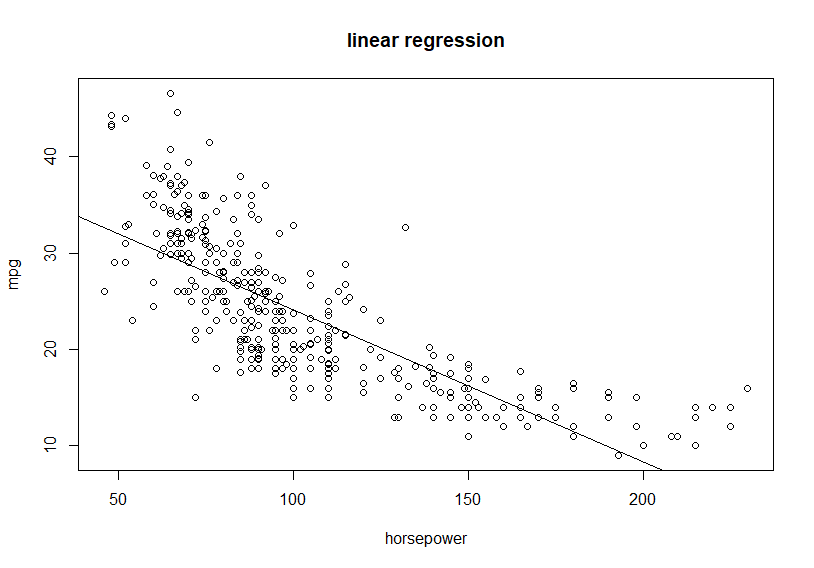
\includegraphics[width=0.8\linewidth]{linear}}
(c.)\\[3ex]
\centerline{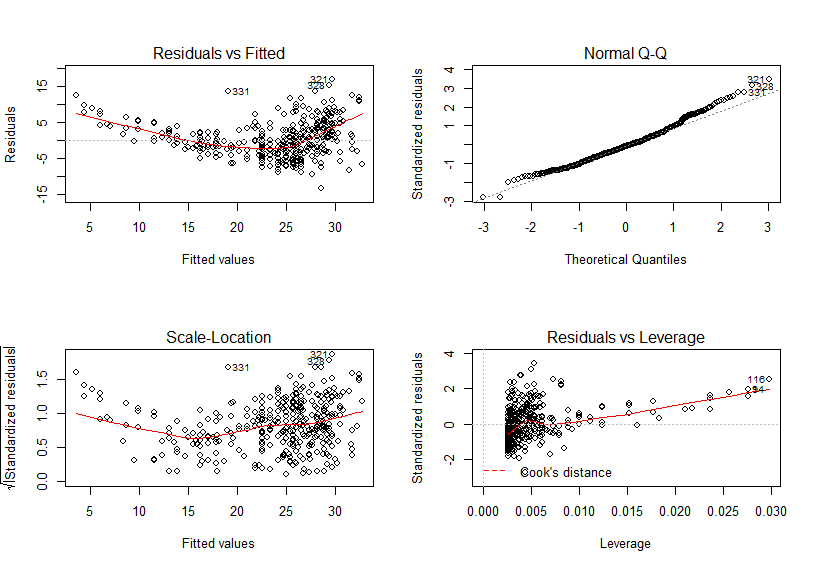
\includegraphics[width=0.8\linewidth]{many}}
\ \\
After standardization, and according to its Q-Q plot, we can discover that the mpg we predict seems Normally distributed. 
\end{itemize}
\end{document}